\section{模型的建立与求解}

\subsection{相似性度量模型}

\subsubsection{度量角度的确立}

在对小学数学应用题的相似性度量过程中,通常会使用两个依据:

\begin{enumerate}
    \item 根据题干文字进行相似性比对,确定两道题目间题面的相似程度。
    \item 通过人工或机器学习的方式为题目根据知识点进行“标签化”,两道题目之间的标签重合越多,则越相似。
\end{enumerate}

实际上,进行“标签化”对题目进行相似性度量是较为科学且准确的,符合师生快速锁定同类题型进行巩固训练的实际需求,而光凭文本信息进行相似性度量的结果并不符合实际的教育需求。

但仅根据少量题目样本无法将“标签化”过程有效自动化,难以避免通过人工手段为题目加上知识点标签。考虑到平台运营的切实情况,人工进行“标签化”操作成本过大,且判断过程中人为主观因素较多,可能也会导致度量结果出现较大偏差。

因而,本文经过综合考虑,还是选择通过题干文字进行相似性比对进行相似性度量。

\subsubsection{度量过程的关键步骤}


本文将度量过程总结成四个关键步骤以便于读者理解,下文也将围绕这四个关键步骤进行展开:

\begin{enumerate}
    \item 文本预处理
    
    文本预处理是自然语言处理中的重要步骤之一,其目的是将原始的文本数据转换成计算机可以处理的形式。为了提高文本处理任务的效率和准确性,文本预处理是在进行后续分析处理的必要前置步骤。

    \item 借助LDA模型建立相似性矩阵
    \item 使用余弦相似度计算相似性结果
\end{enumerate}

\subsubsection{文本预处理}

首先需要对题目文本进行分词处理,以好通过词袋模型的方式将题目文本进行向量化,进行进一步的研究。因本文研究的题目大多处于中文语言环境下,需先对题目进行分词处理。本文为了研究方便,使用的是被广泛使用的开源中文分词工具jieba。另外也可以使用NLPIR分词系统达到相同效果。NLPIR分词系统是由中国科学技术大学自然语言处理与社会人文计算实验室开发的一款中文自然语言处理工具。它是基于统计和规则两种方法相结合的分词系统,能够对中文文本进行精准的分词和词性标注,完美契合本文的研究需要。

在分词处理的过程中,还需要分离并忽略标点符号、数字、停用词等词语的影响。详细的处理操作可以参考周萍老师在《语义分析及相似性度量方法》\cite{ZhouJiYuYuYiFenXiDeWenBenXiangSiXingDuLiangYanJiuJiYingYong2017}研究中总结的预处理流程。但本文简化了处理流程,仅对分词结果进行了简单的标点符号排除与数字排除,以加快研究进程。

\begin{figure}[htbp]
    \centering
    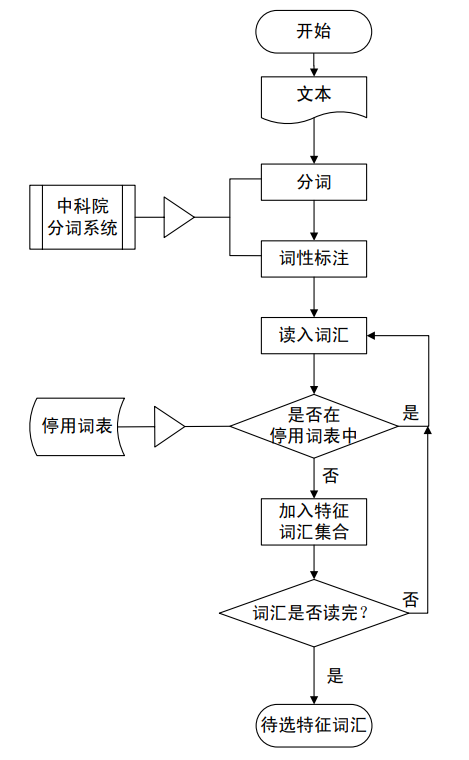
\includegraphics[width=6cm,height=10cm]{res/Text preprocessing process.png}
    \caption{文本预处理流程图}
\end{figure} 

在这里也给出一段进行文字预处理的Python代码以作参考,并作为后续研究的前提:

\begin{mgCodeBlock}[Python 文字预处理代码]
    \VerbatimInput{res/participle.py}
\end{mgCodeBlock}

\subsubsection{借助LDA模型建立相似性矩阵}

若仅通过传统方式进行普通的“文字对比”,可以采取TF-IDF分析文本中的关键词再进行相似性度量。但TF-IDF是通过计算文本中每个词的出现频率和在文档集中的逆文档频率来对文本进行编码的一种手段,在过程中没有“主题”这一概念的考量。如果对长篇文章、论文进行检索,TF-IDF算法可以起到很好的度量效果,但针对文本信息较小的小学数学应用题来说,TF-IDF算法并不能良好的将题目进行归类,分析结果可能因题目背景的改变受到严重限制。

因此,本文选用更适合“题目”这一研究对象的度量模型——LDA模型,进行相似性度量。LDA模型可以将题目集合分解为一组潜在的话题,并确定每个题目的话题分布。这些话题可以被视为题目的主题,因此LDA可以用于识别和分析题目集合中的主题和关键词,并确定题目之间的相似性。

相似的,在“在线编程题目推荐算法”的相关研究中\cite{LuoRongHeZhiShiDianYuTuJuanJiDeZaiXianBianChengTiMuTuiJianSuanFa},也选用了LDA模型作为题目相似性的判断依据之一,可见LDA模型在题目相似性度量上有出色的效果。接下来对LDA模型的介绍,也将围绕这篇论文进行描述。
\begin{figure}[htbp]
    \centering
    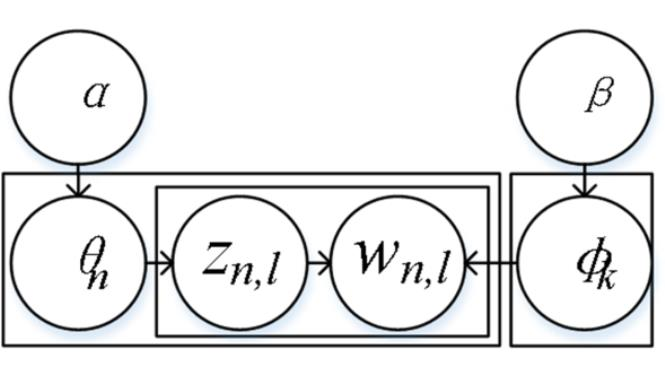
\includegraphics[width=9cm,height=5cm]{res/LDA.jpg}
    \caption{LDA模型图解}
\end{figure} 

如上图所示,LDA 模型假设每个文档都是多个主题的概率分布,每个主题都是多个分词的概率分布,因此文档-分词概率矩阵可以分解为文档-主题概率矩阵与主题-分词概率矩阵。

笔者也为各位读者提供下表以简明介绍上图中符号的意义,并提前说明下文将会使用到的一些符号的意义:

\begin{table}[htbp]
    \centering
    \begin{tabular}{@{}cc@{}}
    \toprule
    符号            & 意义                        \\ \midrule
    $K$           & 主题总数                      \\
    $k$           & 主题编号                      \\
    $Z_{n,l}$     & 文档$n$中第$l$个分词对应的主题编号      \\
    $\alpha$      & 控制文档-主题分布的超参数(狄利克雷分布先验参数) \\
    $\beta$       & 控制主题-词语分布的超参数(狄利克雷分布先验参数) \\
    $w_{n,l}$     & 是文档$n$中第$l$个分词对应的主题编号     \\
    $\theta _{n}$ & 文档$n$的主题分布                \\
    $\varphi_{k}$ & 主题$k$的词汇分布                \\ \bottomrule
    \end{tabular}
\end{table}

接下来,本文将介绍LDA模型的应用过程,该过程也将参考罗文劼与肖梓良老师编写的《融合知识点与图卷积的在线编程题目推荐算法》\cite{LuoRongHeZhiShiDianYuTuJuanJiDeZaiXianBianChengTiMuTuiJianSuanFa}中对LDA模型应用的过程介绍。

首先,在得到给定题目与分词结果的前提下,可以得到$n$与$w_{n,l}$的值。先验参数$\alpha$与$\beta$则采取经验法则,默认设置为$\frac{1}{K}$ 。当然,还有如网格搜索、贝叶斯优化等其他方式选定更优的先验参数,但本文为研究便利,采用较为简单的方式确定先验参数,不采用其他的方式。读者可以根据自身需要尝试选用其他方式确定先验参数。接下来,则使用吉布斯采样法学习LDA模型中的主题分布$\theta _{n}$,过程如下:

\begin{enumerate}
    \item 给定主题总数$K$。
    \item 给每篇文档的每个词汇随机分配主题编号,初始化$Z_{n,l}$。
    \item 利用吉布斯公式对每个词汇进行采样,求出它对应的主题编号,并更新其主题编号$Z_{n,l}$。
    \item 重复上一步骤,直到吉布斯采样收敛或达到迭代次数。
    \item 输出每篇文档的主题分布$\theta _{n}$。
\end{enumerate}

\subsection{基于模糊数学的难度度量模型}

\begin{figure}[h]
    \centering
    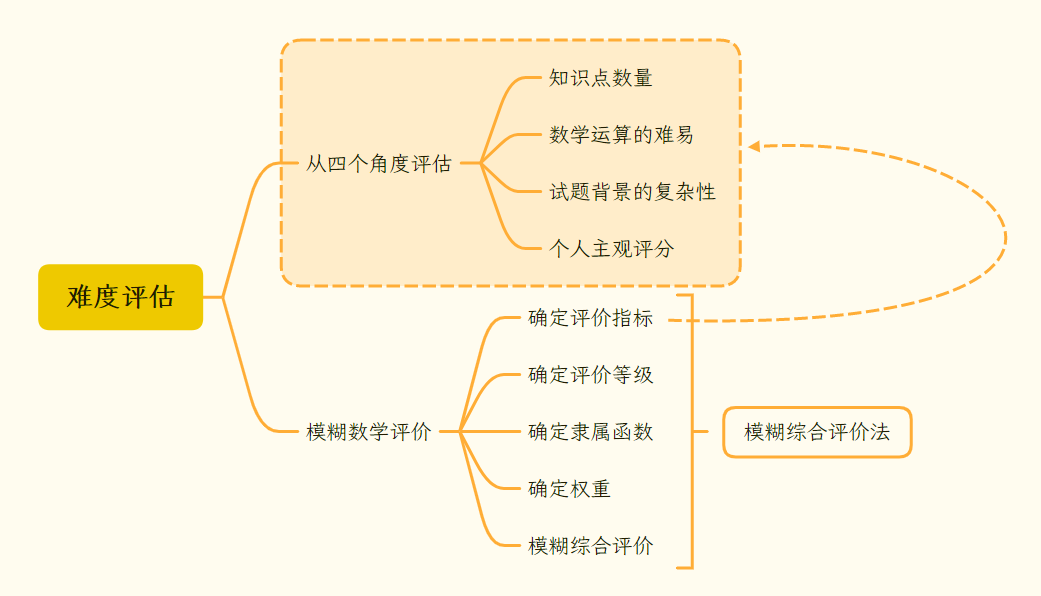
\includegraphics[scale=0.3]{res/figure040041.png}
    \caption{模糊评价思维导图}
\end{figure}

\subsubsection{确定模糊数学理论方法}

对于一个题目来说,其难度与很多因素有关,并且很难量化地用这些因素来表示一个题目的难度,即一个题目的难度只能用模糊的标准来表示,从而让题目难度度量变得十分困难。

除了根据考试的类型度量题目难度之外,还有根据题目的实际得分率确定题目的难度等其他方法。但是这些方法并不能对度量题目难度提供很好的帮助。如果根据题目的实际得分率确定题目难度,需要采集大量真实的试卷信息。此方法难度大、工作量大,很难保证在有限时间内获得准确的信息。为此需要重新思考其他方法,尽可能很好地对题目难度进行度量。

由此,建立了基于模糊数学的难度度量模型。

相对于研究和处理确定性现象的数学理论和方法,模糊数学是研究和处理模糊性现象的一种数学理论和方法\cite{MoHuShuXue}。为了解决题目难度度量十分困难的问题,提出基于模糊数学的难度度量模型。由于模糊数学的特殊性,其在没有精确标准的题目难度度量方面可以起到很好的度量作用。

综上所述,本文采用模糊数学的理论方法对题目难度进行度量。

\subsubsection{分析题目难度影响因素}

对于一个题目来说,有很多因素能够影响其难度。经分析,主要有四个因素对题目难度产生了影响。

首先,影响一个题目难度最深的因素,是该题目所用到的\textbf{知识点数量}。当一道题要求掌握的知识点数量越多时,学生需要掌握越多的知识点才有可能解决这一问题,即对学生解题的要求越高,从而增加题目的难度。

其次是该题目\textbf{数学运算的难度}。在满足学生发挥稳定、有充足时间、不受外界干扰等理想情况下,该题目数学运算越复杂,学生出错的概率越大,写对该题目的概率就越小,进而让该题目越难。

再其次是\textbf{题目背景的复杂性}。如果题目直接把条件和问题表达清楚,那么这个题目就非常明确;然而很多时候题目中会出现含有故事背景、篇幅较长等各种其他情况,使题目条件不清晰,并且需要学生从中挖掘题目条件和问题。这类题目显然相对于上一种来说,难度更大。

最后是教师的\textbf{个人主观难度判断}。教师对题目更加了解,即对题目难度的确定更加准确。但是考虑到对于不同的教师,其资历和阅题数等各方面不同,从而影响到最终的结果,因而将该因素排在最后。

影响题目难度还有其他因素,如学生知识点实际掌握情况,学生考前的学习情况

\subsubsection{确定难度度量指标}

假定\textbf{题目难度度量因素集}$S_{factor}$,且有:
\begin{equation}
    S_{factor} = \{ s_1, s_2, s_3, s_4 \}
\end{equation}

其中$s_1$、$s_2$、$s_3$和$s_4$为四个影响题目难度的因素,分别代表知识点数量、数学运算的难度、题目背景的复杂性和个人主观难度判断。

\subsubsection{确定难度度量等级}

假定\textbf{难度度量等级}集合$S_{level}$,其中$S_{level}(i)$表示某个因素的得分等级为$i$。

等级越高,某个因素对该题目的难度,相较于其他题目同样的因素与对应的题目的难度来说,贡献越大,即题目越难。

经过考虑,划分为五个等级:
$$S_{level} = \{1, 2, 3, 4, 5\}$$
分别对应得分$1, 2, 3, 4, 5$。

\subsubsection{确定题目难度得分矩阵}

假定\textbf{题目难度得分矩阵}$M_{diff}$,其中$M_{diff}(i, j)$表示第$i$题第$j$个因素的得分等级。

因此,对于所有的$i \geq 1, 1 \leq j \leq 4$,有:
$$M_{diff}(i, j)\in S_{level}$$

由于题目难度得分矩阵不确定,并且对于不专业的人来说很难得到准确结果,考虑让多个教师合作完成。

假定有$n$个教师分别完成各自的题目难度得分矩阵,\textbf{所有教师的题目难度矩阵}为一个三维矩阵$M_{diff}'$,其中$M_{diff}'(i, j, k)$表示第$k$个教师认为第$i$题第$j$个因素的得分,且对于所有的$i \geq 1, 1 \leq j \leq 4, 1 \leq k \leq n$,满足:
$$M_{diff}'(i, j, k)\in S_{level}$$

得到每个教师的题目难度得分矩阵后,分别对每一题每个因素求教师数量的平均值,设为最终的题目难度得分矩阵,即:

\begin{equation}
    M_{diff}(i, j) = 
    \frac{
        \sum_{k = 1}^{n}M_{diff}'(i, j, k)
    }{n}
\end{equation}

\subsubsection{确定难度度量权重}

假定\textbf{题目难度因素权重序列}$L_{weight}$,其中$L_{weight}(j)$表示第$j$个元素影响题目难度的权重,并且$1 \leq j \leq 4$。

经分析,考虑:
\begin{equation}
    L_{weight} = [4, 3, 2, 1]
\end{equation}

\subsubsection{计算题目难度值}

构建题目难度度量模型之后,可以由此得到\textbf{难度值}$L_{diff}$,其中$L_{diff}(i)$表示第$i$题的难度值,并且满足$i \geq 1$。

由建立的模型可得对应题目难度的加权值为:
\begin{equation}
    L_{diff}(i) = 
    \sum_{j = 1}^{4} \left [ 
        M_{diff}(i, j) \cdot L_{weight}(j)
    \right ]
\end{equation}

\subsubsection{题目难度模糊综合评价}

由于本题目难度度量模型针对的是附件中题库内的所有题目,对于每一题来说,难度值都是相对于题库内所有题目的难度值而言。

假定题目相较于题库中其他题目的难度为\textbf{难度系数}。所有题目的难度系数序列为$L_D$,其中$L_D(i)$表示第$i$题的难度系数,且有$i \geq 1$。

则难度系数的计算方式为:

\begin{equation}
L_D(i) = 
    \frac{
        L_{diff}(i) - \min L_{diff}
    } {
        \max L_{diff} - \min L_{diff}
    }
\end{equation}

其中$\max L_{diff}$为题库中题目最大的难度值、$\min L_{diff}$为题库中题目最小的难度值,并且有$0 \leq L_D(i) \leq 1, i \geq 1$。

至此,题库中所有题目的难度均度量完成,即$L_D$。

\subsection{模型的应用举例——对附件1题库的分类}



\subsection{模型的应用举例——对附件2的难度分析}



% ============================================================
%
% 模型的评价与改进
%
% ============================================================

\section{模型的评价与改进}

\subsection{模型的优点}

\begin{itemize}
    \item 
\end{itemize}

\subsection{模型的缺点}

\subsection{模型的改进}